\documentclass[a4paper, 12pt]{article}

\usepackage[T1]{fontenc}
\usepackage[polish]{babel} 
\usepackage[utf8]{inputenc} 
\let\lll\undefined
\usepackage{setspace}
\usepackage{fancyhdr}
\usepackage{hyperref}
\usepackage{pdfpages}
\usepackage{listings}
\usepackage{color}
\usepackage{graphicx}
\usepackage{enumitem}
\usepackage{latexsym}
\pagestyle{fancy} 
\hypersetup{
    colorlinks=true,
    linkcolor=blue,
    filecolor=magenta,      
    urlcolor=cyan,
}
\usepackage{geometry}
\newgeometry{tmargin=2.5cm, bmargin=2.5cm, lmargin=2.5cm, rmargin=2.5cm} 
\newcommand{\mainmatter}{\clearpage \cfoot{\thepage\ of \pageref{LastPage}}
\pagenumbering{arabic}} 
\lstset{language=bash}  
\begin{document}

	\begin{titlepage}

\includegraphics[width = 40mm]{logo.jpg}
		\begin{center}
    			\vspace{3cm}
    					\Large\textit{\textbf{Procesy biznesowe (definicje, kryteria i klasyfikacje, przykłady)}}
   			\vspace{4cm}
		\end{center} 

		\hfill\begin{minipage}{0.54\textwidth}
			\Large Wykonali:\newline
				1. Ivan Prakapets 295139 \newline
				2. Aliaksandr Karolik 295138
		\vspace{\baselineskip}
		\end{minipage}
		
		\hfill\begin{minipage}{0.54\textwidth}
			\Large Sprawdzający:\newline
		 		prof.dr hab.inż.Andrzej Dzieliński
\vspace{\baselineskip}
		\end{minipage}

		\hfill\begin{minipage}{0.54\textwidth}
			\Large Data:10.11.2019
			\vspace{\baselineskip}
		\end{minipage}
	\end{titlepage}
\newpage
\mainmatter
\setlength{\headheight}{15pt}
\doublespacing
\tableofcontents
\newpage

\linespread{0.5}
\setlist{nolistsep}

\section{Wstęp}
\hspace*{1.5 cm}Poniższy dokument jest  pracą semestralną na temat "Procesy biznesowe (definicje, kryteria i klasyfikacje, przykłady)". W tym dokumencie postaramy się zdefiniować co to jest proces biznesowy oraz zbadać jakie są kryteria i klasyfikacji procesów biznesowych. Również postaramy się rozpatrzyć kilka procesów biznesowych w różnych firmach aby na ich podstawie zaobserwować różne rodzaje procesów biznesowych. 
\section{Definicja procesu biznesowego}
\hspace*{1.5 cm}Poniżej zostaną zaprezentowane różne definicje pojęcia proces biznezosy:

\hspace*{1.5 cm}Proces biznesowy jest zbiorem czynności, ma jeden lub więcej rodzajów wejść i tworzy wartość wyjściową dla klienta. Proces biznesowy posiada swój cel, a oddziałują na niego zdarzenia zachodzące w świecie zewnętrznym lub w innych procesach.
(Hammer and Champy 1993)

\hspace*{1.5 cm} Proces biznesowy jest to zbiór powiązanych procedur lub działań, które wspólnie zapewniają osiągnięcie celu biznesowego lub celu polityki, zwykle w ramach struktury organizacyjnej definiującej funkcjonalność ról i zależności pomiędzy nimi. (Workflow Management Coalition 1999) 

\hspace*{1.5 cm}Proces biznesowy może być postrzegany jako struktura czynności zaprojektowanych na działania nakierowane na klienta końcowego i dynamiczne zarządzanie przepływami związanymi z produktami, informacją, środkami finansowymi, wiedzą i wizją.(Stock and Lambert 2001)        

\hspace*{1.5 cm}Proces biznesowy lub inaczej metoda biznesowa, która funkcjonuje w każdym przedsiębiorstwie. Są to zadania ze sobą powiązane, które prowadzą do osiągnięcia wyznaczonego efektu. Najważniejszym celem tego procesu jest zrozumieć klienta, dostawców i słabe strony tego procesu.(A. Bitkowska 2009, s.26)

\hspace*{1.5 cm}Określony zbiór czynności biznesowych, które stanowią niezbędne kroki w celu osiągnięcia celu biznesowego. Obejmuje on przepływ i użycie informacji oraz zasobów.(Object Management Group – BPMN v. 2.0 2011) 
\paragraph{Podsumowanie czym jest proces biznesowy}\mbox{}\\
%\subsection{Podsumowanie czym jest proces biznesowy} 
\hspace{1.5 cm} Bazując na powyższych definicjach, można przyjąć, że proces biznesowy, to zbiór powiązanych ze sobą czynności, które przekształcają wejścia w wyjścia według określonych reguł, w oparciu o określone zasoby i w efekcie prowadzą do dostarczenia klientowi produktu/usługi realizując tym samym cele biznesowe organizacji.
\section{Kryteria i klasyfikacje procesów biznesowych}
\hspace*{1.5 cm}W literaturze  można  spotkać  wiele  różnych  kryteriów  podziału  i klasyfikacji  procesów.  I  tak,  według  M.  Portera  [Porter,  1985,  s.  23]  wyróżnić  można  dwa  podstawowe  rodzaje  procesów:  \textbf{podstawowe}  i  \textbf{pomocnicze}. Do procesów podstawowych zaliczył on: 
\begin{itemize}
	\item Logistykę „na wejściu”, która obejmuje działania związane z przygotowaniem produkcji,
	\item wytwarzanie produktu, 
 	\item logistykę  „na  wyjściu”,  która obejmuje  działania związane ze sprzedażą,
	\item marketing,
	\item usługi posprzedażne.
\end{itemize}

\hspace*{1.5 cm}Natomiast wśród pomocniczych wymienił procesy związane z: 
\begin{itemize}
	\item Zarządzaniem całą jednostką,
	\item zarządzaniem zasobami ludzkimi,
	\item zaopatrzeniem,
	\item rozwojem mającym na celu doskonalenie produktów i procesów.
\end{itemize}

\hspace*{1.5 cm} Z  kolei  R.S.  Kaplan  i  R.  Cooper  [Kaplan,  Cooper,  2001, s.  99],  [Kaplan, Cooper, 2000, s. 200] wyróżnili procesy:
\begin{itemize}
	\item Innowacyjne – związane z określaniem rynku docelowego oraz two-rzeniem oferty produktu (usługi), 
	\item operacyjne  –  dotyczące  wytwarzania  produktu  (usługi)  i  dostarcza-nia go klientowi,
	\item obsługi posprzedażnej – obejmujące obsługę klienta po dostarczeniu mu produktu,
\end{itemize}
\hspace*{1.5 cm} Oraz podzielili je na:
\begin{itemize}
	\item Konieczne – których wykonanie jest niezbędne do dostarczenia war-tości  i  których  nie  można  obecnie  poprawić,  uprościć,  zredukować czy wyeliminować, 
	\item istotne – dostarczające wartość, aczkolwiek możliwe jest ich uprosz-czenie i poprawienie,
	\item nieistotne – które powinny być wyeliminowane. 
\end{itemize}
\hspace*{1.5 cm} Z kolei najobszerniejszą klasyfikację procesów przedstawiła organizacja APQC (American Productivity Quality Center), która przygotowała Model Klasyfikacji Procesów (z ang. Process Classification Framework PCF). Wspomniana  organizacja  zaproponowała  wprowadzenie  12  kategorii procesów, które podzielone zostały na dwie grupy:
\begin{itemize}
	\item Procesy  operacyjne  –  traktowane  jako  kluczowe,  dla  danego  podmiotu gospodarczego, 
	\item procesy  wspomagające  –  stanowiące  wsparcie  dla  procesów  operacyjnych.
\end{itemize}
\hspace*{1.5 cm} Do  pierwszej  grupy  zaliczono  5  kategorii  charakteryzujących  działalność  podmiotu  decydujących  o  zakresie  funkcjonowania przedsiębiorstwa,  natomiast  do  procesów  wspomagających  zakwalifikowano  7 kategorii,  które  przenikają  wszystkie  procesy  podstawowe  i  jednocześnie są podstawą do wydzielania ich na zewnątrz (outsourcing). Ilustrację  graficzną  klasyfikacji  procesów  zgodnej  z  modelem  APQC  przed-stawia tablica 1.

\begin{table}[h]
	\begin{center}
		\scalebox{1}{\begin{tabular}{ | l | l | }
				\hline
				Proces & Charakterystyka \\ \hline
				Operacyjne & 1.0 - Opracowanie wizji i strategii \\
						   & 2.0 - Rozwój i zarządzanie produktami i usługami  \\
						   & 3.0 -  Marketing i sprzedaż produktów i usług \\ 
						   & 4.0 - Zaopatrzenie, realizacja i dostawa produktów/usług \\
						   & 5.0 - Zarządzanie obsługą klienta		   \\ \hline
				Wspomagające & 6.0 -Organizacja i zarządzanie 	kapitałem ludzkim \\
				             & 7.0 - Zarządzanie technologią informatyczną\\
				             & 8.0 - Zarządzanie zasobami finansowymi\\
				             & 9.0 - Nabywanie, budowa i zarządzanie mieniem \\
				             & 10.0 - Zarządzanie ochroną środowiska oraz bezpieczeń-stwem i higieną pracy \\
				             & 11.0 - Zarządzanie relacjami zewnętrznymi\\
				             & 12.0 -  Zarządzanie wiedzą, doskonaleniem i zmianą\\
				\hline
		\end{tabular}}
	\end{center}
	\caption{\label{tab:bolts} Klasyfikacja procesów według modelu APQC}
\end{table}
\hspace*{1.5 cm}Model APQC nie ogranicza się do przedstawienia listy 12 kategorii procesów,  rozwija  się  proponując  następującą  zależność:  kategoria  procesów  –  grupa  procesów  –  procesy  –  czynności  (działania).																																														
\section{Przykłady biznes procesów w różnych rodzajach firm}
\subsection{Biznes procesy w firmie IT}
\subsubsection{Opis ogólny procesu}
\hspace*{1cm} Potrzebujemy zakupić nowe serwery z potrzeby zaspokojenia bieżącego zapotrzebowania na moc obliczeniową, przyrostu danych oraz wymiana obecnie posiadanego systemu na nowszy, bo jest brak kompatybilności z nowymi systemami operacyjnymi, brak wsparcia producenta, z tego wynika wysokie ryzyko awarii. Poniżej jest dokładne opisane problemy, informacje, wykresy oraz charakterystyki dotyczące obecnych i nowych serwerów.\newline
\subsubsection{Występujące problemy w firmie} 
		\begin{itemize}
		        \item Na obecnym serwerze baza danych wzrasta się około 100 Gb co rok. Ze względu na duże przyrosty danych na obecnych serwerach brakuje miejsca. Brak przestrzeni na dane powoduje coraz wolniejsze działanie serwera. W przypadku awarii niemożliwym staje się szybka naprawa. W obecnej postój pracy wynosi 5 dni.
	        	\item Problemy z komunikacją oraz transferem danych między serwerami spowodowana przestarzałością sprzętu.
	        	\item Niski poziom Uptime, poziom dostępności systemu określony w procentach. Informujący o czasie ciągłego i bezawaryjnego działania serwerów w ciągu roku. Można spodziewać się awarii w niedługim okresie.
	        	\item Okres gwarancji na sprzęt oraz oprogramowanie wygasł, wiąże się to z częstrzą możliwością występowania corac cięższych awarii.
	        	\item Przestarzały sprzęt wycofany już z produkcji i powszechnego użytku. Posiadany sprzęt zurzywa się i traci pierwotą niezawodność. Generuje to ryzyko braku możliwości wymiany części i podzespołów w przypadku uszkodzeń i awarii.
	        	\item  Stare oprogramowanie traci swoją kompatybilność z nowymi systemami i ma słabsze możliwości względem nowych.
	        	\item Niewystarczająca moc obliczeniowa powoduje powolną pracę serwerów. Dane przesyłane do aplikacji są coraz wolniej selekcjonowane oraz generowanie z długim czasem oczekiwania na wyniki. Wpływ na to ma szybkość procesowa, pamięć RAM, pojemność dysku, przepustowość, itp.
		    \end{itemize}
	  \subsubsection{Wnioski z problemów} 
	
			 	\hspace*{1cm} Pozostaje mało miejsca i istnieje potrzeba rozszerzenia przestrzeni roboczej poprzez podłączenie dodatkowych urządzeń pamięci masowej lub zwiększenie pojemności istniejącej macierzy dyskowej. Niestety uniemożliwia to przestarzały sprzęt niekompatybilny z odpowiednikami dostępnymi na rynku.\newline
			\hspace*{1cm}  Wszystkie powyższe problemu powodują przerwy, awarie oraz  przestoje - \textbf{generuje to straty materialne oraz oszczerbki na reputacji firmy.}\newline
			Poniższe diagramy pokazują zurzycie przestrzeni dyskowej dwóch serwerów.\newline
			
\includegraphics[width=1.1\textwidth]{diagram_dyski_1}
			
\includegraphics[width=1.1\textwidth]{diagram_dyski_2}
			
			Poniższe diagramy przedstawiają użyteczność procesora i odczytu fizyczne-go/logicznego.
			  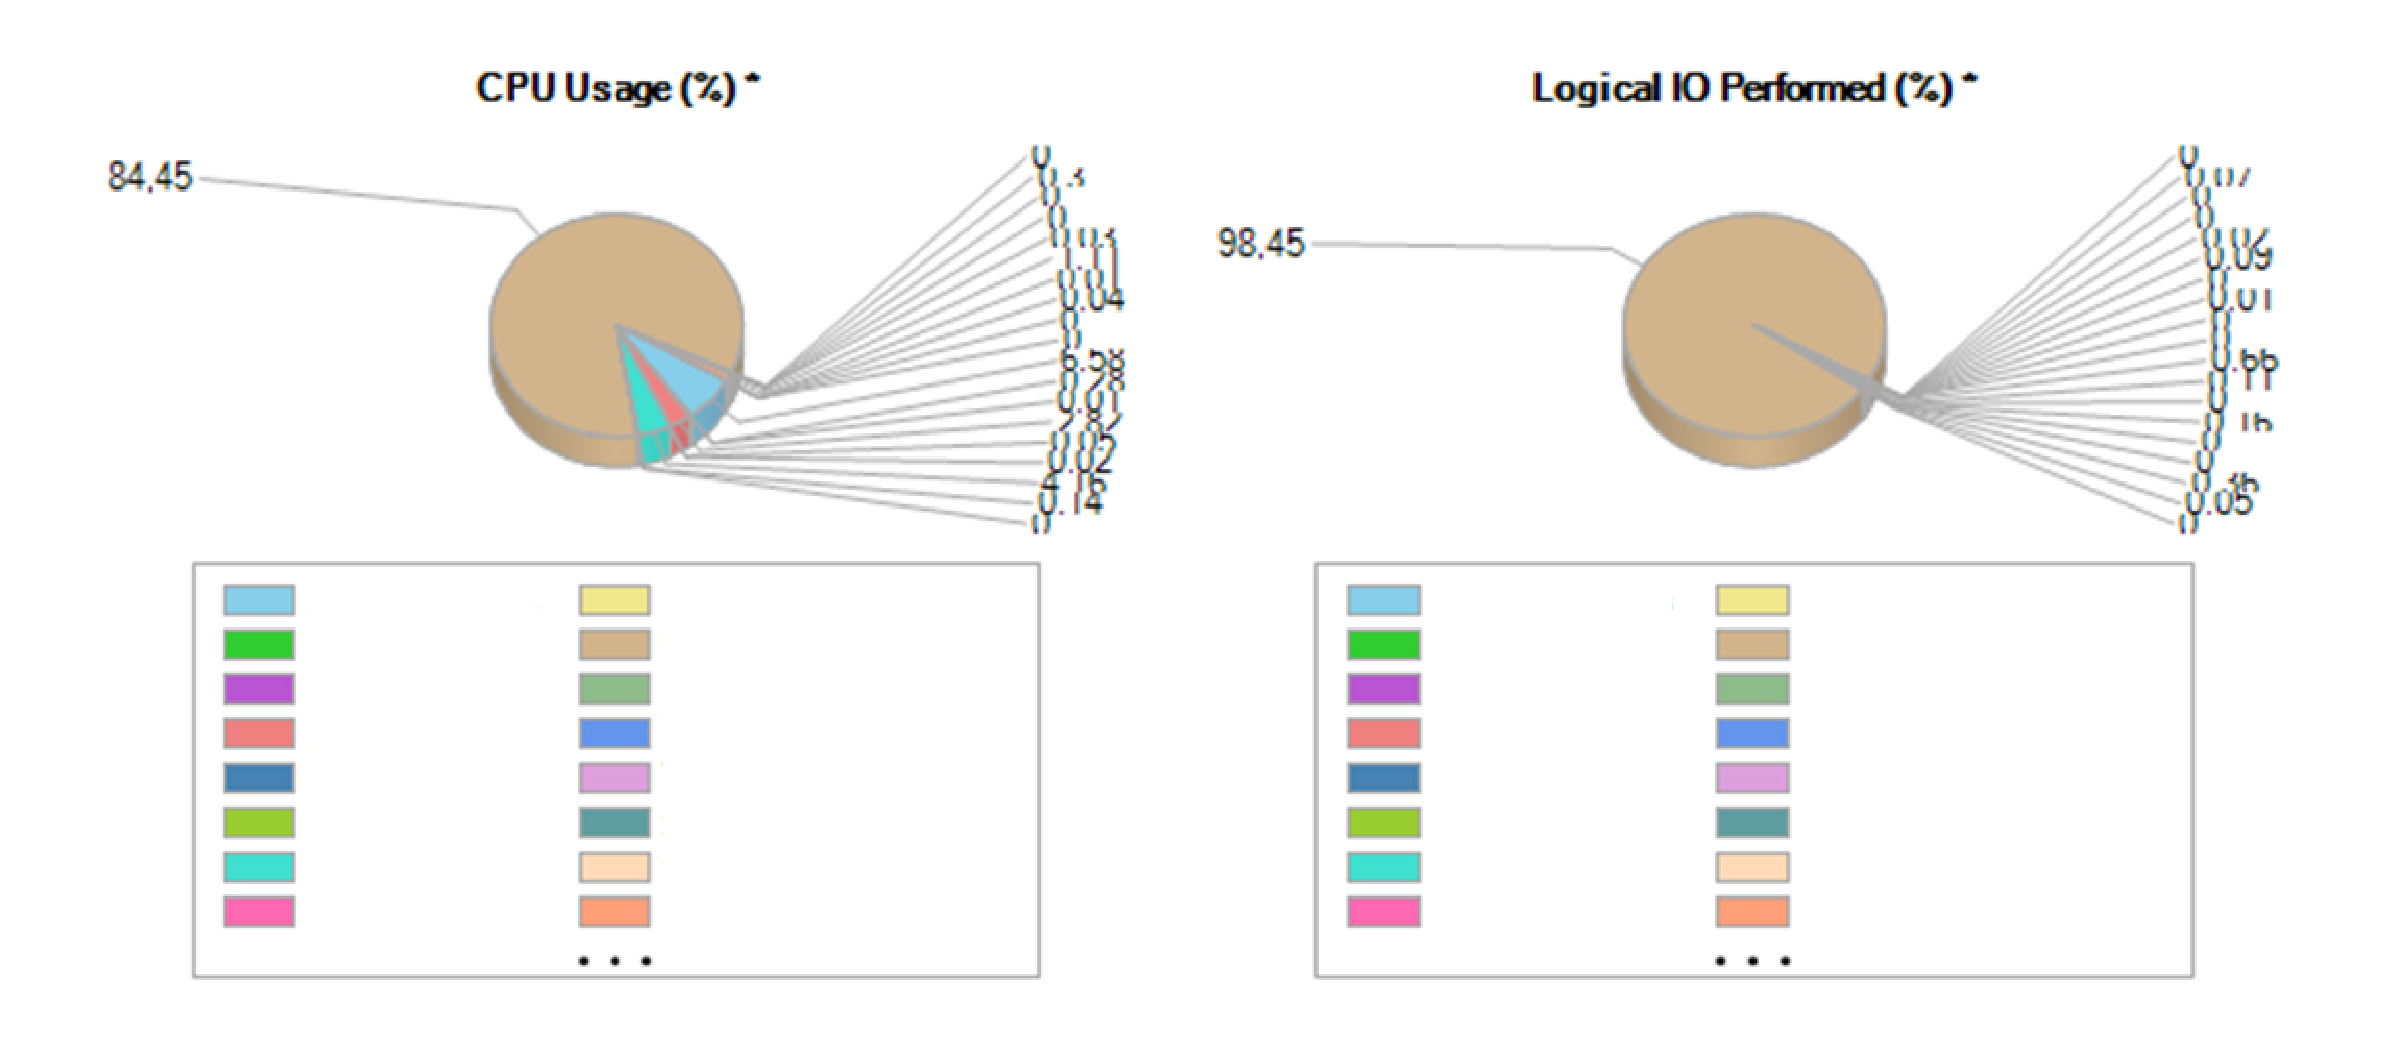
\includegraphics[width=1.0\textwidth]{diagram}. \newline
			\hspace*{1cm} Odczyty fizyczne pokazują, ile stron SQL Serwer musiał odczytać z dysku, aby spełnić żądanie. Odczyty logiczne pokazują, ile stron SQL Serwer musiał odczytać z pamięci podręcznej, aby spełnić żądanie. 
			\subsubsection{Rozwiązanie problemów}
				\subsubsection{Obecny stan}
			  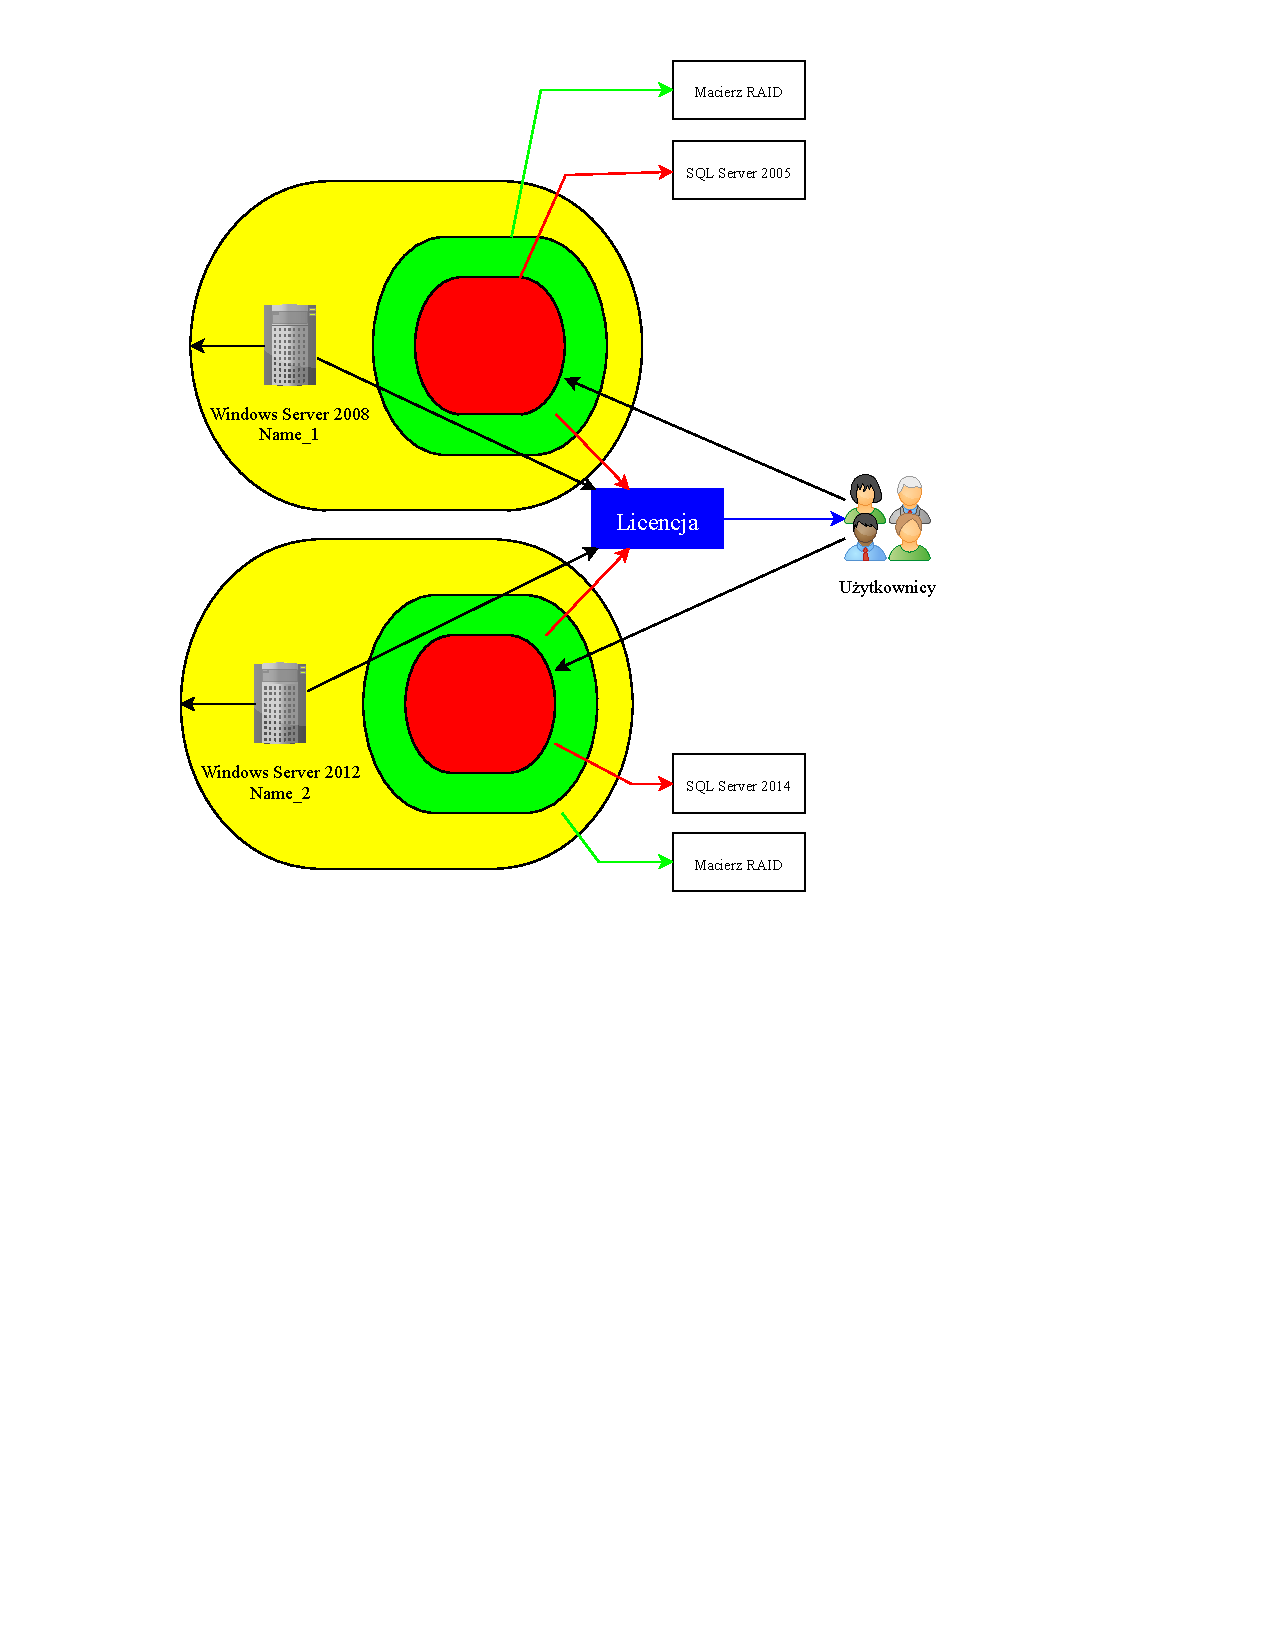
\includegraphics[scale=0.7]{obecny_stan}
			  
			  	\subsubsection{Proponowany stan}
			  	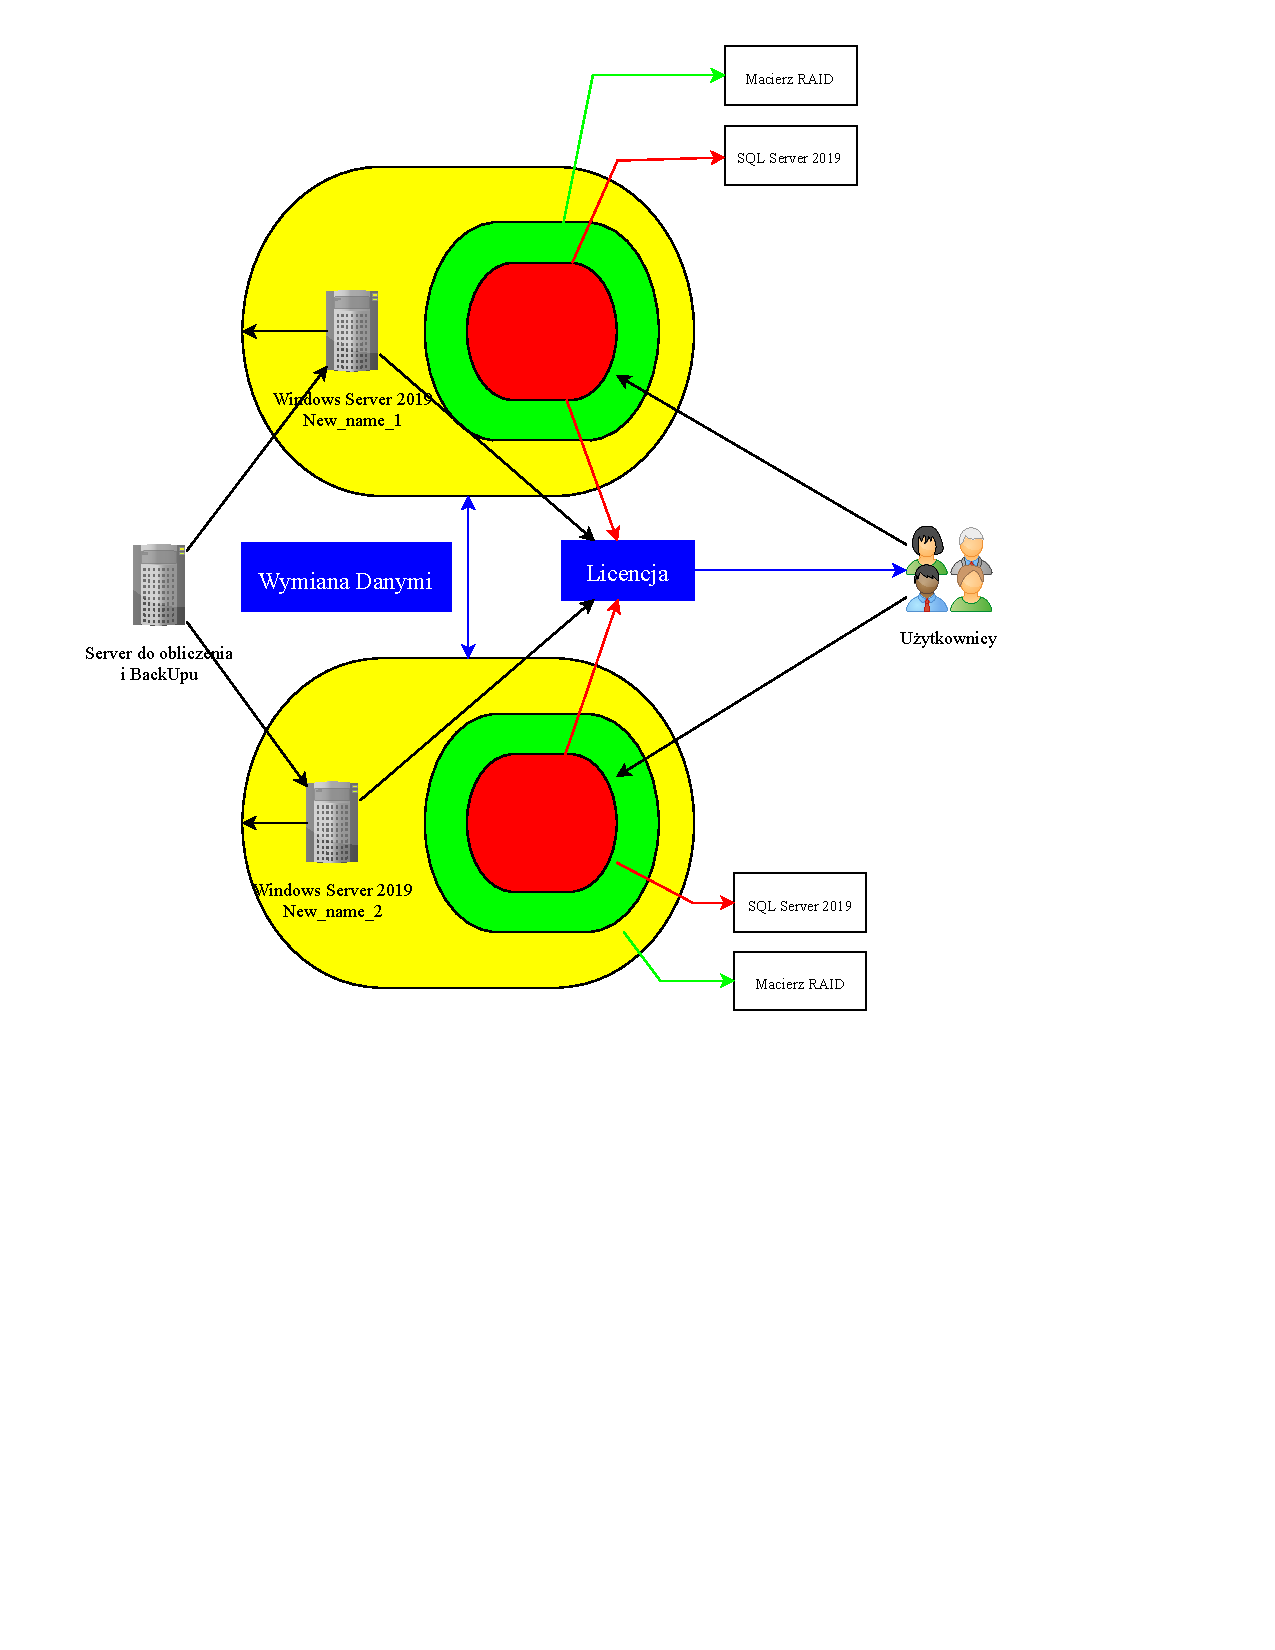
\includegraphics[scale=0.7]{proponowany_stan} \newline
			  	\subsubsection{Opis przepływu procesu biznesowego}
			  	\hspace*{1cm} W internecie można znaleść wiele rankingów porównujących serwery. Poniżej kilka przykładowych: \newline
				\href{https://www.crn.com/slide-shows/data-center/300106536/the-10-top-enterprise-servers-of-2018-so-far.htm/1} {Top Enterprise Servers 2018} \newline
				\href{https://www.techradar.com/news/best-small-business-servers} {Serwery 2019}\newline
				\href{https://www.skapiec.pl/cat/93-serwery/ranking.html} {Ranking Serwerów}\newline
				\hspace*{1cm}Po przeprowadzonej analizie firm oraz charakterystyk poszczególnych serwerów wybraliśmy \texttt{DELL PowerEdge} jako najlepsze rozwiązanie dla naszej firmy. Najlepszyn rozwiązaniem jest zakupienie 3 nowych serwerów.
				
Serwer ma zawierać: 
				\begin{itemize}
\item Procesory 2 * \textbf{Intel® Xeon® Gold 6126}.Jeden procesor posiada moc obliczeniową \textbf{31 GFLOPS}. 
							\begin{itemize}
\item Obecnie nie wystarcza mocy obliczeniową dla wszystkich zadań. Ten procesor zmniejsza zużycia energii i zwiększa efektywność przetwarzania wielu zadań.
							\end{itemize}
\item  Serwer zawiera w sobie 16 rdzeni i obsługuje do 512 GB, ale potrzebujemy pamięć \textbf{RAM 32GB}
							\begin{itemize}
\item Obecnie mamy mało pamięci RAM, która jest nie wystarczająca dla realizacji wszystkich zadań.
							\end{itemize}
\item Dyski \textbf{ 6 * 1.2TB SAS} dla przechowywania danych  oraz BackUp'ów  + dyski \textbf{2 * 800GB SSD SAS} do wykonywania operacji obliczeniowych ze względu na jego szybkość. Łącznie \textbf{8.8TB} 
								\begin{itemize}
\item Obecnie mamy łącznie 2.2 TB pamięci i przestrzeń ta została prawie całkowicie wykorzystana.
								\end{itemize}
\item Zapotrzebowanie na 3 serwery : dwa serwery do klasterów oraz jeden do obliczeń i BackUpów.
				\end{itemize}			
				\subsubsection{Klastry SQL Server 2019} 	
	\hspace*{1cm} Klastry to technologia, która pozwala łączyć kilka systemów komputerowych w całość. 
Cel klastra to z duplikowanie  serwerów i zapewnienie nieprzerwanego funkcjonowania aplikacji. W serwerach bazodanowych wszystkie informacje są zapamiętywane na każdej równolegle pracującej maszynie. W razie awarii systemy i urządzenia łączą się działającym serwerem, zawierającym te same dane.
\newline
	\hspace*{1cm}Klastry SQL Server 2019 to nowy sposób wykorzystania SQL Server do tworzenia wartościowych baz relacyjnych i przechowywania dużych zbiorów danych na jednej, skalowalnej platformie. Dzięki temu analiza danych oraz aplikacje łączące się z bazą są bardziej elastyczne i działają wydajniej. Duże klastry danych SQL Server 2019 zapewniają kompletną platformę i pomagają zwiększyć sukces  organizacji.
\subsubsection{Wnioski} 
	\hspace*{1cm} Rozwiązaniem minimalnym jest zakup 2 serwerów pozwalających na zabezpieczenie firmy w razie awarii serwera głównego. Biorąc pod uwagę zobowiązania związane z dyrektywą RODO należy pamiętać o należytym zabezpieczeniu i przetwarzaniu danych osobowych pracowników, partnerów oraz klientów firmy, należy dodatkowo zabezpieczyć się przed wyciekami danych i zalecane jest odseparowanie portalu CMS od pozostałych systemów bazodanowych. Najlepszym rozwiązanie jest kupienie 3 serwerów oraz dodatkowych dyski w celu zwiększenia dostępnej przestrzeni masowej. Pozwoli to na nie na zwiększenie przestrzeni ale również mocy obliczeniowej niezbędnej do prawidłowej pracy systemów i aplikacji firmy oraz tworzenia raportów i analiz na podstawie danych zawartych w systemach bazodanowych. Należy również pamiętac o dodatkowym zabezpieczeniu jakim jest cyklinczne kopiowanie danych na zewnętrzne media lub nośniki. Daje to gwarancję bezpieczeństwa i odtworzenie systemu nawet w razie nadzwyczajnych sytuacji jak pożar itp..

\subsection{Biznes procesy w firmach marketingowych}
\subsubsection{Wstep}
\hspace*{1 cm} W tym rozdziale zostaną opisane procesy biznesowe zachodzące w firmach marketingowych. Zostaną również opisane przyczyny, dlaczego te procesy zachodzą i co one rozwiązują. Przykładowe procesy zachodzące w firmach marketingowych:
\begin{itemize}
	\item Opracowanie planu marketingowego,
	\item opracowanie strategii promocyjnej.
\end{itemize}
\subsubsection{Biznes proces o nazwie 'Opracowanie planu marketingowego'}
\paragraph{Ogólny opis procesu}\mbox{}\\
\hspace*{1 cm}Plan marketingowy firmy ma kluczowe znaczenie przy planowaniu działań, wraz z budżetem, planem produkcji i planem sprzedaży. Roczny plan przedsiębiorstwa, odpowiednio, określa ogólne cele przedsiębiorstwa, jednak plan marketingowy ma większe znaczenie nad innymi częściami ogólnego planu rocznego, ponieważ:
\begin{enumerate}
	\item Cele planu marketingowego mają bezpośredni wpływ na wyniki innych części planu rocznego,
	\item decyzje zapisane w planie marketingowym określają, co dokładnie wyprodukuje firma, po jakiej cenie i gdzie sprzedać, jak się reklamować.
\end{enumerate}
\hspace*{1 cm}Plan marketingowy służy jako kluczowy przewodnik dla pracy personalu zajmującego się działaniami związanymi z marketingiem w firmy.
\paragraph{Problemy które proces rozwiązuje}
\begin{itemize}
	\item Firma rozwija się spontanicznie, od zwycięstwa do porażki,
	\item konflikty w programach rozwoju firmy,
	\item firma losowo kupuje produkty, stara się zdywersyfikować ofertę produktową w momencie, gdy wymagana jest koncentracja na głównej ofercie produktowej.
\end{itemize} 
%\newpage
\paragraph{Opis przepływu procesu biznesowego}\mbox{}\\
\hspace*{1 cm} Główne cele, które firma chcę osiągnąć przy tworzeniu planu marketingowego następujące:
\begin{itemize}
	\item Systematyzacja, formalny opis pomysłów liderów firmy, przekazywanie ich pracownikom,
	\item ustalanie celów marketingowych, zapewniając kontrolę nad ich osiągnięciem,
	\item koncentracja i rozsądny podział zasobów firmy.
\end{itemize} 
\hspace*{1 cm} Proces składa się z sześciu kroków:
\begin{enumerate}
	\item Definicja misji przedsiębiorstwa,
	\item analiza SWOT,
	\item definiowanie celów i strategii organizacji jako całości,
	\item określenie zadań i programu działań dla ich realizacji,
	\item opracowanie planu marketingowego i monitorowanie jego realizacji,
	\item budżetowanie na potrzeby wdrożenia planu marketingowego.
\end{enumerate}
Więcej szczegółów na temat kroków:
\begin{enumerate}
	\item Na etapie definicji misji przedsiębiorstwa określa się cel wszystkich późniejszych obszarów w których firmy może działać.
	\item Analiza SWOT daje jasny obraz tego, gdzie znajduje się firma i co ona ma wewnątrz: analiza mocnych i słabych stron przedsiębiorstwa, a także szans i zagrożeń związanych z bezpośrednim otoczeniem przedsiębiorstwa (środowisko zewnętrzne);
	\item Trzecia sekcja stanowi podstawę do opracowania konkretnego programu działań marketingowych. Ten etap planu marketingowego obejmuje prognozowanie rozwoju rynków docelowych (segmentów), dynamikę procesów makro i mikroekonomicznych, a także możliwości zasobów przedsiębiorstwa. Na podstawie powyższej analizy wyznaczane główne cele  przedsiębiorstwa. Cele reprezentowane są w ustrukturyzowanym drzewie celów, w korzeniu którego znajduje się globalny cel firmy.
	\item Na czwartym etapie zadania działu marketingu są określane w ramach ogólnego planu przedsiębiorstwa i opracowywany jest program działań w celu rozwiązania tych problemów. Dla każdego docelowego segmentu rynku należy zaplanować odpowiednie towary (usługi) o wymaganej jakości i ilości, ich cenach, punktach sprzedaży i taktykach promocji dla konsumenta.
	\item Piąty krok pozwala uzyskać sam dokument, z określanymi wartościami parametrów, za pomocą których będzie monitorowana realizacja planu marketingowego.
	\item Budżet marketingowy-część planu marketingowego, która odzwierciedla planowane wartości przychodów, kosztów i zysków. Wysokość dochodu jest uzasadniona prognozowaną wielkością sprzedaży. Koszty są definiowane jako suma wszystkich rodzajów kosztów. Zatwierdzony budżet stanowi podstawę do zapewnienia produkcji towarów i działań marketingowych.
\end{enumerate}



\subsubsection{Biznes proces o nazwie 'Opracowanie strategii promocyjnej'}
\paragraph{Ogólny opis procesu}\mbox{}\\
\hspace*{1 cm}Strategia promocji - to zbiór wszystkich środków, za pomocą których przedsiębiorstwo przekazuje otoczeniu informacje o swojej działalności, produktach i usługach. Przez promocję rozumie się oddziaływanie na odbiorców produktów polegające na przekazywaniu im informacji, które mają zwiększać wiedzę na temat towarów firmy i samej firmy w celu stworzenia dla nich preferencji na rynku.
\newline \hspace*{1 cm}Celem promocji jest przekazanie klientom docelowym informacji, że produkt jest dostępny w odpowiednim miejscu po odpowiedniej cenie. Strategia to plan gry, który umożliwia osiągnięcie przez firmę założonych celów. (Kotler P., 2005)
\paragraph{Problemy które proces rozwiązuje}
\begin{itemize}
	\item Zwiększenie sprzedaży produkcji,
	\item wzrost popytu (na przykład z sezonowym spadkiem sprzedaży),
	\item poprawa konkurencyjności firmy,
	\item Wprowadzenie firmy na rynek.
\end{itemize}
%\newpage
\paragraph{Opis przepływu procesu biznesowego}\mbox{}\\
\hspace*{1 cm}Strategia promocyjna musi być przygotowana w sposób profesjonalny i metodyczny. Aby przyniosła ona odpowiedni efekt, musi opierać się na sześciu etapach:
\begin{enumerate}
	\item Identyfikacja lub wyznaczanie określonego rynku docelowego.
	\newline Pierwszy i najważniejszy etap, od którego zależy powodzenie promocji. Polega on na identyfikacji potencjalnych nabywców produktów danej firmy. Przedsiębiorstwo powinno tak skierować swoją kampanię, aby dotarła ona do trafnie dobranych adresatów, czyli do potencjalnych klientów firmy.
	
	Pomagają w tym badania marketingowe, dzięki którym firma dowiaduje się, kto jest najczęściej nabywcą ich produktów.

	\item Wyznaczenie celów promocji.
	\newline Wyróżnia się dwa najważniejsze cele promocji:
	\begin{itemize}
		\item Informacyjne – powinny wyprzedzać cele sprzedażowe, ale w praktyce są one najczęściej realizowane łącznie z nimi. Cele informacyjne to dążenie, aby jak największa część rynku została poinformowana o istnieniu danej firmy i jej ofercie,
		\item sprzedażowe – dążenie do osiągnięcia jak największego wolumenu sprzedaży produktów długofalowych.
	\end{itemize}
	\item Ustalenie budżetu promocji.
	\newline Firma musi wydzielić określone środki przeznaczone na kampanię promocyjną, gdyż od tego zależy jak długo będzie trwała kampania i jak bardzo będzie profesjonalna. Budżet powinien być dostosowany do wielkości rynku docelowego, celów kampanii promocyjnej, specyfikacji promowanych produktów oraz stanu konkurencji w danej branży.
	
	Istnieje kilka sposobów wyznaczania budżetu promocji:
	\begin{itemize}
		\item "Tyle, ile trzeba" – na kampanię przeznacza się tyle środków ile potrzebne jest do zrealizowania celów promocji.
		\item "Tyle, ile może" – stosowana przez mniejsze firmy, które mają dokładnie określoną ilość środków na kampanię.
		\item "\ Za procesją", – przeznaczenie na kampanię promocyjną tyle środków, ile przeznaczają konkurenci, po to by zapobiec eliminacji naszej firmy z rynku.
	\end{itemize}

	\item Wybór kanału promocyjnego.
	\newline Wybór kanału promocyjnego opiera się na wyborze odpowiednich masmediów do upowszechniania kampanii promocyjnej, tak aby dotrzeć do, jak największej liczby potencjalnych klientów.
	Każda firma może wybrać kanał, jakim jest telewizja, radio elektroniczne lub teleinformatyczne media promocyjne np.: Internet, kino, teatry, billboardy itp.
	
	Telewizja to jeden z najlepszych sposobów reklamy, ponieważ łączy elementy ruchu obrazu scenografii, muzyki, słowa i gry aktorskiej. Wiąże się to jednak z wysokim kosztem.
	
	Radio może przekaz promocyjny zaadresować do wybranej, selektywnej grupy klientów, dlatego tak popularne są reklamy radiowe.
	
	Media drukowane mają swoje zalety (niska cena, łatwość zamieszczenia reklamy, duża elastyczność kampanii promocyjnej) i wady (krótki żywot reklamy w gazecie codziennej, łatwość zaginięcia reklamy w gąszczu ogłoszeń). Dużą popularnością cieszą się reklamy umieszczone w miesięcznikach, ponieważ są to czasopisma najczęściej skierowane do określonej grupy klientów.
	
	\item Przygotowanie i wykonanie kampanii promocyjnej
	\newline Na tym etapie należy rozwiązać następujące problemy:
	\begin{itemize}
		\item Co chcemy przekazać,
		\item jak zwerbalizować ten pomysł,
		\item jak odpowiednio użyć sloganów,
		\item kto ma to powiedzieć.
		
	\end{itemize}
	\item Pomiar wyników produkcji
	\newline Pomiar wyników produkcji opiera się na sprawdzeniu, czy kampania przyniosła oczekiwane efekty, czy nie. Porównujemy wielkość sprzedaży przed kampanią, w trakcie i po jej zakończeniu. Jednym z celów promocji może być budowa pozytywnego wizerunku firmy lub przełamanie negatywnego wizerunku.
		
\end{enumerate}









\subsection{Zarządzanie procesami biznesowymi w sektorze hotelarskim}
\subsubsection{Wstep}
\hspace*{1 cm} W tym rodziałe zostaną opisane zarządzanie procesami biznesowymi w hotelach: z naciskiem na zapewnienie wysokiej jakości obsługi gości\newline
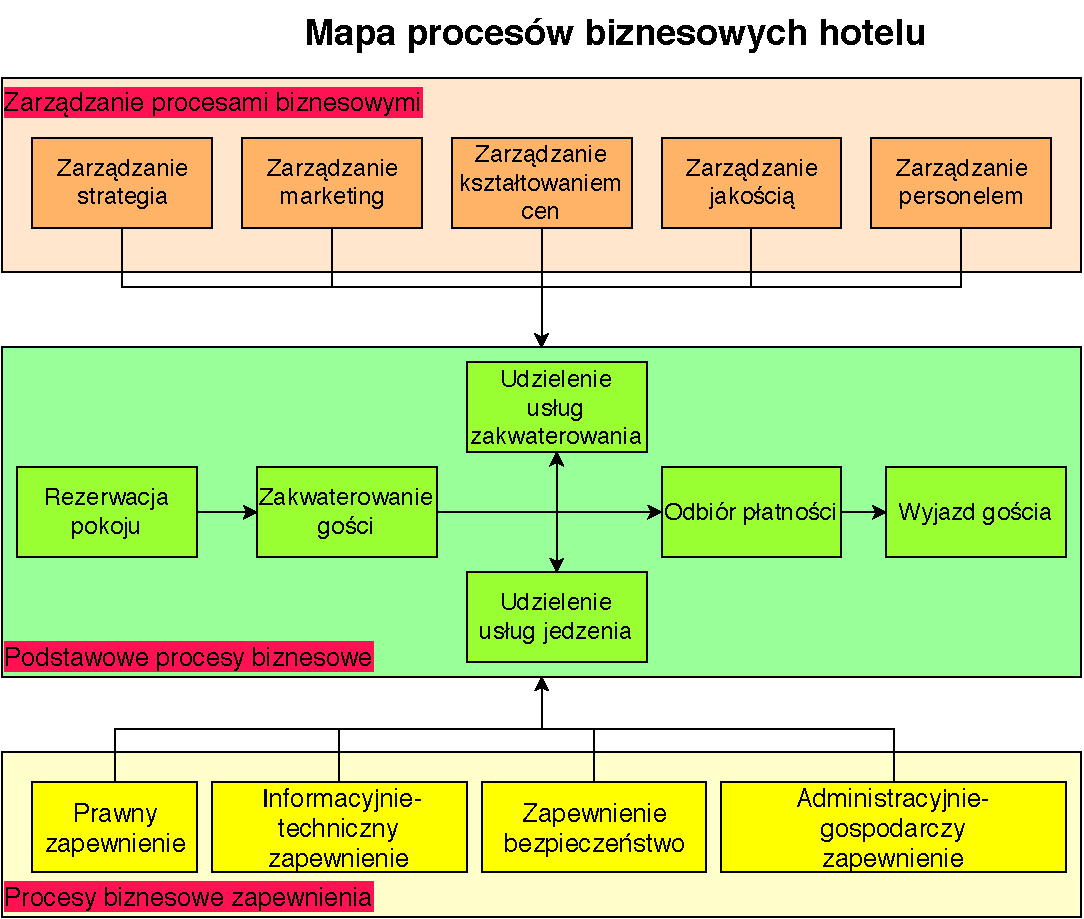
\includegraphics[scale=0.9]{hotel} \newline
Powyższa mapa opisuję podstawowe etapy w sektorze hotelarskim, aby zrozumieć listę i hierarchię procesów. Mapa procesów biznesowych pozwala wyróżnić procesy biznesowe najwyższego poziomy i rozdzielić wszystkie procesy na grupy. Każdy problem może być powiązany z określonym procesem biznesowym lub kilkoma procesami.\newline
Każdy etap jest analizowany, a usprawnienia procesów biznesowych są stosowane.\newline
\hspace*{1cm}Firmy zmuszone są do szybszego wprowadzania innowacji w swoich modelach biznesowych. Muszą skupić się na klientach, konkurencji i procesach. Te nowe modele biznesowe zostały opisane jako „Innowacyjne technologie stosowane w branży hotelarskiej biznes”.



\subsubsection{Procesy biznesowe w sektorze hotelarskim}
Branża hotelarska jest prezentowana każdego dnia jako globalna branża z właścicielami i klientami na całym świecie. Korzystanie z usług hotelowych, takich jak: zakwaterowanie, restauracja, bar, centrum spa nie jest już uważane za luksus. Dzisiaj wszystkie te usługi są niezbędne wielu osobom w ich codziennym życiu.\newline

\subsubsection{Innowacyjne technologie stosowane w branży hotelarskiej}
\paragraph{Wstęp}\mbox{}\\
\hspace*{1cm}Innowacje w sektorze hotelarskim to system organizacyjny, ekonomiczny, badawczy, technologiczny i inny wydarzenia mające na celu całkowitą odnowę usług turystycznych w szczególny mechanizm jego wdrażania i promocji w celu osiągnięcia efektu ekonomicznego, społecznego lub innego. Branża hotelarska odgrywa ważną rolę rola w gospodarce kraju. W niektórych krajach jest to najważniejsza pozycja dochodów w budżecie państwa 
\paragraph{Innowacje technologiczne.}\mbox{}\\
\hspace*{1cm} USB gniazda. Obecnie prawie wszyscy są wyposażeni w wystarczająco dużą liczbę przenośnych urządzeń elektronicznych, takich jak:
odtwarzacze mp3, smartfony, tablety, aparaty fotograficzne i kamery wideo. Dla wygody klienta, aby nie nosił ze sobą różnych adapterów i adapterów, proponuje wyposażać swoje pokoje w specjalne gniazda USB. Te gniazda mogą mieć 2 modyfikacje:
\begin{enumerate}
	\item specjalistyczne gniazda USB;
	\item combo gniazda USB z tradycyjnymi złączami.
\end{enumerate}
\paragraph{Antichrapkowy pokój}\mbox{}\\
\hspace*{1cm} Skuteczność proponowanej innowacji polega na całkowitej izolacji akustycznej pomieszczenia, to znaczy, że pokój jest wyposażony w specjalną pochłaniającą dźwięk głowicę łóżka, poduszki anty-chrapkowe i podszewki pod plecami.
\paragraph{Chipy elektroniczne do pościeli w pokojach hotelowych}\mbox{}\\
\hspace*{1cm} Chipy mają na celu zapobieganie kradzieży przez gości ręczniki hotelowe, poszewki na poduszki i prześcieradła. Technologia polega na tym, że do bielizna hotelowej jest wydobywane chipy identyfikacyjnych o częstotliwości radiowej,które są wszyte w szwach wyrobów włókienniczych i informują hotelarzy, wysyłając sygnał w postaci syreny o próbie wyprowadzenia rzeczy poza hotel.


\subsubsection{Pozostawanie w fazie zarządzania zaproszeniami gości i skargami}
\paragraph{Ogólny opis procesu}\mbox{}\\
\hspace*{1cm} Podczas procesu obsługi gości dział front office powinien upewnić się, że goście są zadowoleni podczas pobytu. Kiedy goście mają jakieś specjalne wymagania, zwykle proszą o pomoc w recepcji. Może to dotyczyć: napraw pokoju, dodatkowych udogodnień w pokoju lub informacji. Jeśli te skargi lub prośby zostaną szybko rozwiązane, poprawia to zadowolenie gościa, a tym samym przyczynia się do świadczenia wysokiej jakości obsługi gości.
\paragraph{Definicja problemu.}\mbox{}\\
\hspace*{1cm} Po pierwsze, należy zauważyć, że w obu przypadkach (prośba i skarga) żaden hotel nie wypełnia żadnego raportu i nie przekazuje do odpowiedniego kierownika pod koniec zmiany na prośby i problemy napotkane podczas pracy. Po drugie, recepcjonista nie otrzymuje żadnych informacji zwrotnych od gospodyni domowej ani konserwacji, jeśli akcja została wykonana pomyślnie. Nie mając żadnych informacji, personel recepcji nie jest w stanie odpowiedzieć na wymagania gości.
\paragraph{Sugestie dotyczące ulepszeń}\mbox{}\\
\hspace*{1cm} Recepcjonista powinien przygotować raport z problemami pod koniec godzin pracy, w tym wnioski klientów i reklamacje, które napotkano podczas ich zmiany.

\paragraph{Oczekiwane wyniki}\mbox{}\\
\hspace*{1cm} Raport pomaga gromadzić dane, a następnie analizować je w celu rozwiązania problemów. Gdy raporty te są odpowiednio monitorowane, mogą przyczynić się do podjęcia odpowiednich środków w celu podniesienia jakości usług świadczonych gościowi.

\subsubsection{Wnioski}
\hspace*{1cm} Obecnie na rynku usług hotelowych brakuje wysokiej jakości obiektów noclegowych, na które jest duży popyt usługi.
Analizując działalność przedsiębiorstw hotelowych w warunkach globalizacji należy zwrócić uwagę na ciągłą walkę o klienta, w wyniku której opracowywane są innowacyjne pomysły i procesy doskonalenia przedsiębiorstwa hotelarskiego.

Zastosowanie zarządzania procesami biznesowymi zapewnia wiele korzyści dla firm w usługach hotelowych. Istnieje wiele różnych procesów, takich jak dostarczanie niezbędnych danych wejściowych, proces obsługi klienta, sprzątanie i sprzątanie, proces jedzenia i napojów itp. Badanie to miało na celu usprawnienie obsługi biura obsługi przez biznes podejście do zarządzania procesami.
\section{Literatura}
\begin{thebibliography}{}
	\bibitem{litlink1}  Porter M. (1985), Competitive Advantage, Free Press, New York. 
	\bibitem{litlink1} Kaplan R.S., Cooper R. (2001), Strategiczna karta wyników. Jak przełożyć strategię na działanie, Wydawnictwo Naukowe PWN, Warszawa. 
	\bibitem{litlink1} Sitek  T.,  Gola  M.,  Klasyfikacja  metod  modelowania  procesów  biznesowych,  [w:] Wachowicz  J.  (red.),  Problemy  wykorzystania  informatyki  w  zarządzaniu,  Wydawnictwo Politechniki Gdańskiej, Gdańsk 2005, s. 7-20.
	\bibitem{litlink1} Auksztol J., Chomuszko M. (2012), Modelowanie organizacji procesowej,
Wydawnictwo Naukowe PWN, Warszawa. 
	\bibitem{litlink1} Grajewski P. (2012), Procesowe zarządzanie organizacją, Polskie Wydawnictwo Ekonomiczne, Warszawa. 
	\bibitem{litlink1} Kotler P., (2005), Marketing, Poznań
	\bibitem{litlink1} Michael Havey, Essential Business Process Modeling, O'Reilly Media, 2005;
	\bibitem{litlink1} Diagramy robione ręcznie w draw.io
	\bibitem{litlink1} R. Szubstarski, Rynek się rozkręca. Raport z rynku hotelarskiego w Polsce, „Hotelarz” 2012
	\bibitem{litlink1} Armisted C., Rowland P., Managing Business Processes, Wiley
and Sons, Chichester. 
	\bibitem{litlink1} Grajewski P. (2012), Procesowe zarządzanie organizacją, Polskie Wydawnictwo Ekonomiczne, Warszawa. 
	\bibitem{litlink1} Cerović, Z. (2010) Hotelski menadžment, Sveučilište u Rijeci
	\bibitem{litlink1} Rutherford, D., O’Fallon, M. (2010) Hotel Management and Operation, John Wiley and Sons, Inc
	\bibitem{litlink1} Stutts, A.T., Worton, J.F. (2006)  Hotel and Lodging  Management: An  Introduction, John Wiley and Sons, Inc
	\bibitem{litlink1} Weske,  M. (2012)  Business  process  management –  concepts,  languages,  architectures, Second edition, Springer
	\bibitem{litlink1} Harmon, P. (2005) Business Process Change: A Manager’s Guide to Improving, Redesigning, and Automatic Processes, Morgan Kaufmann Publishers, San Francisco, CA.
	\bibitem{litlink1} Mapa procesów biznesowych jest własnością prywatną robiona ręcznie za pomocą draw.io
	\bibitem{litlink1} Własne doświadczenie w branży IT.
	\bibitem{litkink1} Część własnych pomysłów dla innowacji w sektorze hotelarskim.	 
\end{thebibliography}
\label{LastPage}~
\label{LastPageOfBackMatter}~		
\end{document}